\section{Dämpfung, Verstärkung, Dezibel}

Hinweis: Neben Dezibel gibt es ein weiteres Dämpfungs-/ bzw. Verstärkungsmass: Neper $\mathrm{Np}$
Auf dieses Mass wird allerdings nicht genauer eingegangen. Skript: S.207


\subsection{Dämpfungsfaktor $D$}{206}

Das Verhältnis zwischen Eingangs- und Ausgangssignal wird als Dämpfungsfaktor $D$ bezeichnet

\begin{minipage}[c]{0.3\columnwidth}
    $$ \boxed{ D_P = \frac{P_1}{P_2} } $$
\end{minipage}
\hfill
\begin{minipage}[c]{0.3\columnwidth}
    $$ \boxed{ D_U = \frac{U_1}{U_2} } $$
\end{minipage}
\hfill
\begin{minipage}[c]{0.3\columnwidth}
    $$ \boxed{ D_I = \frac{I_1}{I_2} } $$
\end{minipage}

Die Indizes $U, \, P, \, I$ stehen für die \textbf{Effektivwerte} von Spannung, Leistung und Strom.


\subsection{Dämpfungsmass $a$ in Dezibel}{206}

Durch \textbf{logarithmieren} des Dämpfungsfaktors $D$ erhält man das Dämpfungsmass $a$

\begin{minipage}[c]{0.3\columnwidth}
    $$ \boxed{ a_P =  10 \cdot \log_{10} \Big( \frac{P_1}{P_2} \Big) } $$
\end{minipage}
\hfill
\begin{minipage}[c]{0.3\columnwidth}
    $$ \boxed{ a_U = 20 \cdot \log_{10} \Big( \frac{U_1}{U_2} \Big) } $$
\end{minipage}
\hfill
\begin{minipage}[c]{0.3\columnwidth}
    $$ \boxed{ a_I = 20 \cdot \log_{10} \Big( \frac{I_1}{I_2} \Big) } $$
\end{minipage}


\subsubsection{Umrechnung Verstärkungsfaktor -- Dezibel}

$$ \boxed{ \mathrm{dB} = 10 \cdot \log_{10} (v) \, \Leftrightarrow \, v = 10^{\frac{\mathrm{dB}}{10}} } $$


\subsection{Rechenregeln mit Dezibel}

\begin{itemize}
    \item Faktoren multiplizieren \textrightarrow Dezibel-Werte addieren
    \item Faktoren dividieren \textrightarrow Dezibel-Werte subtrahieren
\end{itemize}


\subsection{Spannungsverstärkungsfaktor}{209}

Hält man sich strikt an die Definition des Verstärkungsfaktors bzw. die Definition der Dezibel, so würde man für Dämpfungen positive
Dezibel-Werte erhalten und für Verstärkungen entspreched negative Dezibel-Werte. Dies ist gegen die Intuition des Ingenieurs. \\
Somit wurde der \textbf{Spannungsverstärkungsfaktor} $\boldsymbol{T_U}$ definiert. Analog zum Dämpfungsmass $a$ wird ein 
\textbf{Verstärkungsmass} $\boldsymbol{g_U}$ definiert.

\begin{minipage}[c]{0.48\columnwidth}
    $$ \boxed{ T_U = \frac{U_2}{U_1} } $$
\end{minipage}
\hfill
\begin{minipage}[c]{0.48\columnwidth}
    $$ \boxed{ g_U = 20 \cdot \log_{10} \Big( \frac{U_2}{U_1} \Big) } $$
\end{minipage}


Aus dieser Definition folgt für die Dezibel-Werte:

\begin{itemize}
    \item \textbf{Verstärkung: } ($U_2 > U_1$) \textrightarrow positive Dezibel-Zahl
    \item \textbf{Dämpfung: } ($U_2 < U_1$) \textrightarrow negative Dezibel-Zahl
\end{itemize}


\example{Kaskadiertes System}{209}

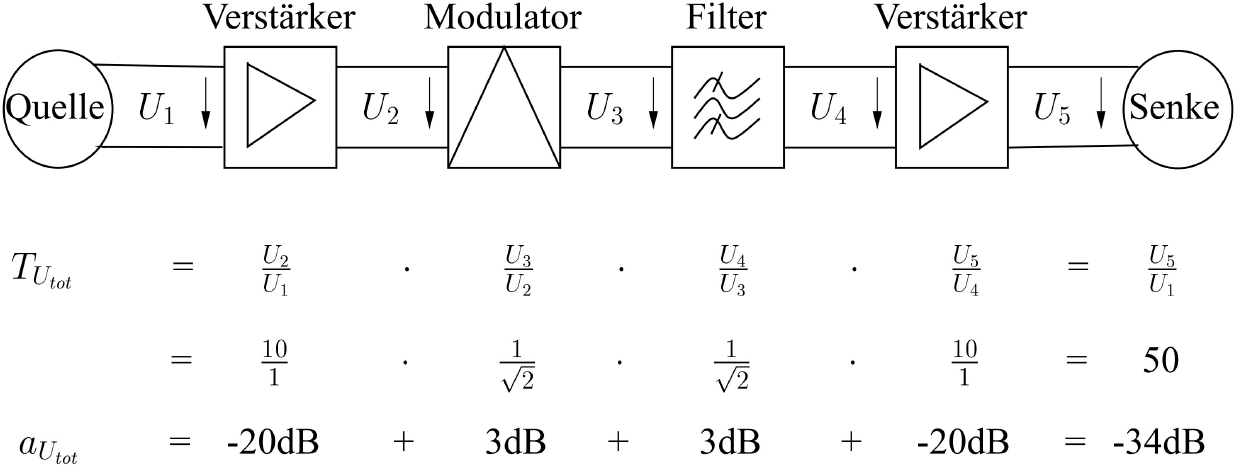
\includegraphics[width=0.9\columnwidth]{images/kaskadierung_verstaerkung_daempfung.png}

Formuliert mit dem Verstärkungsmass $g$ ergeben sich umgekehrte Vorzeichen:
$$ g_{U_{tot}} \quad = \quad - 20 \, \mathrm{dB} \quad  + \quad 3 \, \mathrm{dB} \quad + 
    \quad 3 \, \mathrm{dB} \quad - \quad 20 \, \mathrm{dB} \quad = \quad -34 \, \mathrm{dB} $$



\subsection{Umrechnungs-Tabelle Dezibel -- Faktor}

\textbf{Vorgehen:} Gesuchten $\mathrm{dB}$-Wert als Summe / Differenz von bekannten Werten darstellen 
\textrightarrow Summanden in Faktoren 'transferieren' und multiplizieren / dividieren \\

\textbf{Vorgehen:} Gesuchten Faktor als Produkt / Quotent von bekannten Werten darstellen 
\textrightarrow Faktoren in Summanden 'transferieren' und addieren / subtrahieren \\


\begin{tabular}{ | c | c |}
    \toprule
    \textbf{Dezibel}        & \textbf{Faktor} \\
    \midrule
    $100 = 10 \cdot 10$     & $10 + 10$ \\ 
    $12$                    & $2 \cdot 2 \cdot 2 \cdot 2 = 16$ \\
    $\cor{10}$              & $\cor{10}$ \\
    $9 = 3 + 3 + 3$         & $2 \cdot 2 \cdot 2 = 8$ \\
    $8 = 5 - 3$             & $3.2 \cdot 2 = 6.4$ \\
    $7 = 10 -3$             & $\frac{10}{2} = 5$ \\
    $6 = 3 + 3$             & $2 \cdot 2 = 4$ \\
    $5 = 15 - 10$           & $\frac{32}{10} = 3.2 = \sqrt{10}$ \\
    $4 = 10 - 6 = 10 - 3-3$ & $\frac{10}{2 \cdot 2} = 2.5$ \\
    $\cor{3}$               & $\cor{2}$ \\
    $2= 12-10= 5-3$         & $\frac{16}{10} = 1.6$ \\
    $1 = 10 - 3 - 3 - 3$    & $\frac{10}{2\cdot 2 \cdot 2} = \frac{5}{4} = 1.25$ \\
    $\cor{0}$               & $\cor{1}$ \\
    $-1$                    & $\frac{4}{5} = 0.8$ \\
    \bottomrule
\end{tabular}


\subsection{Relativer und Absoluter Pegel}{210}

Bei den bisher ausgeführten Pegeln handelt es sich um \textbf{relative Pegel}. Im Gegensatz dazu beziehen sich
\textbf{absolute Pegelangaben} immer auf eine Referenzgrösser (erzeugt von einem Normengenerator, siehe Skript). 

% not according to guidelines but \dezibel had issues before... 
\renewcommand{\arraystretch}{1.7}
\begin{tabular}{c c c}
    $(L_U)_{\text{rel}} = 20 \cdot \log_{10} \Big( \frac{U_2}{U_1} \Big)$ & &
    $(L_U)_{\text{abs}} = 20 \cdot \log_{10} \Big( \frac{U_2}{774.6 \, \mathrm{mV}} \Big)$ \\
    
    $(L_I)_{\text{rel}} = 20 \cdot \log_{10} \Big( \frac{I_2}{I_1} \Big)$ & &
    $(L_I)_{\text{abs}} = 20 \cdot \log_{10} \Big( \frac{I_2}{1.291 \, \mathrm{mA}} \Big)$ \\
    
    $(L_P)_{\text{rel}} = 10 \cdot \log_{10} \Big( \frac{P_2}{P_1} \Big)$ & &
    $(L_P)_{\text{abs}} = 10 \cdot \log_{10} \Big( \frac{P_2}{1 \, \mathrm{mW}} \Big)$ \\
\end{tabular}
\renewcommand{\arraystretch}{1}


\subsubsection{Kennzeichnung absoluter Pegel}

\begin{tabular}{ll c ll}
    \textbf{Notation}       & \textbf{Bezugsgrösse} & & 
    \textbf{Notation}       & \textbf{Bezugsgrösse} \\
    $\mathrm{dBW}$          & $1 \, \watt$          & & 
    $\mathrm{dBm}$          & $1 \, \milli \watt$ \\
    $\mathrm{dBV}$          & $1 \, \volt$          & & 
    $\mathrm{dB \micro V}$  & $1 \, \micro \watt$ 
\end{tabular}
